\documentclass[margin=0.5mm]{standalone}
\usepackage{pgfplots}
\usetikzlibrary{pgfplots.groupplots}
\pgfplotsset{compat=1.7}

\definecolor{rred}{RGB}{234,98,255}
\definecolor{ccian}{RGB}{98,140,255}
\definecolor{yyellow}{RGB}{255,205,98}

\begin{document}
	\thispagestyle{empty}

		\centering
		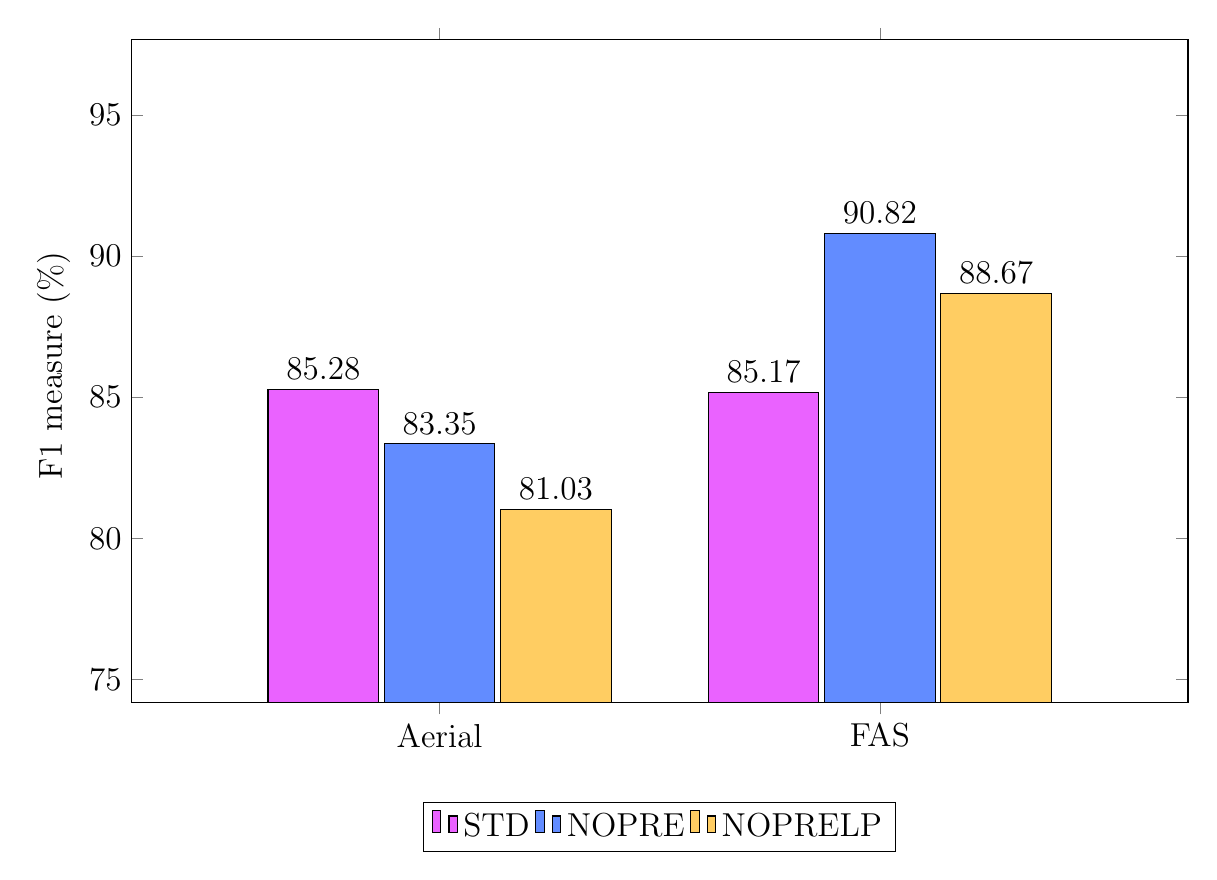
\begin{tikzpicture}
		\begin{axis}[
		width=15cm,
		height=10cm,
		ybar,
		enlargelimits=0.70,
		legend style={at={(0.5,-0.15)},
			anchor=north,legend columns=-1},
		ylabel={\ F1 measure (\%)},
		symbolic x coords={Aerial,FAS},
		xtick=data,
		nodes near coords,
		nodes near coords align={vertical},
		bar width=40pt,
		style={font=\large}		
		]
%					STD		NPRE	NPRE4K
%			Aerial	85.28	83.35	81.03
%			FAS		85.17	90.82	88.67
			
		\addplot [color=black,fill=rred] coordinates {(Aerial,85.28) (FAS,85.17)  };
		\addplot [color=black,fill=ccian] coordinates {(Aerial,83.35) (FAS,90.82) };
		\addplot [color=black,fill=yyellow] coordinates {(Aerial,81.03) (FAS,88.67) };
		
		\legend{STD,NOPRE,NOPRELP}
		\end{axis}
		\end{tikzpicture}
		%\vspace{-0.7cm}
		%\caption{Left: the pitch distribution for the 10 male speakers. Right: the active speech level for the 20 speakers.}\label{fig:pitch}
		%\vspace{-0.5cm}

\end{document}